\documentclass[12pt, a4paper]{article}

\usepackage[a4paper, margin=0.85in, headheight=16pt]{geometry}
\usepackage{graphicx}
\usepackage{fancyhdr}
\usepackage{lastpage}
\usepackage{float}
\usepackage[hidelinks]{hyperref}

\pagestyle{fancy}
\fancyhf{}
\fancyhead[L]{\footnotesize Amir Atef - 24P0310}
\fancyhead[C]{\footnotesize Web Development - CSE343}
\fancyhead[R]{\footnotesize Lab \#5}
\fancyfoot[C]{\footnotesize Page \thepage\ of \pageref{LastPage}}
\renewcommand{\headrulewidth}{0.4pt}
\renewcommand{\footrulewidth}{0pt}

\begin{document}

% ---  Cover Page ---
\thispagestyle{empty}
\vspace*{\fill}
\begin{center}
    {\LARGE \textbf{Web Development - CSE343}}\\[1.5cm]
    {\Large \textbf{Lab \#5 Task}}\\[2.0cm]
    {\large Amir Atef - 24P0310}
\end{center}
\vspace*{\fill}
\clearpage

% ---  Screenshots ---
\section*{Screenshots}
\vspace{0.4cm}

\begin{figure}[H]
    \centering
    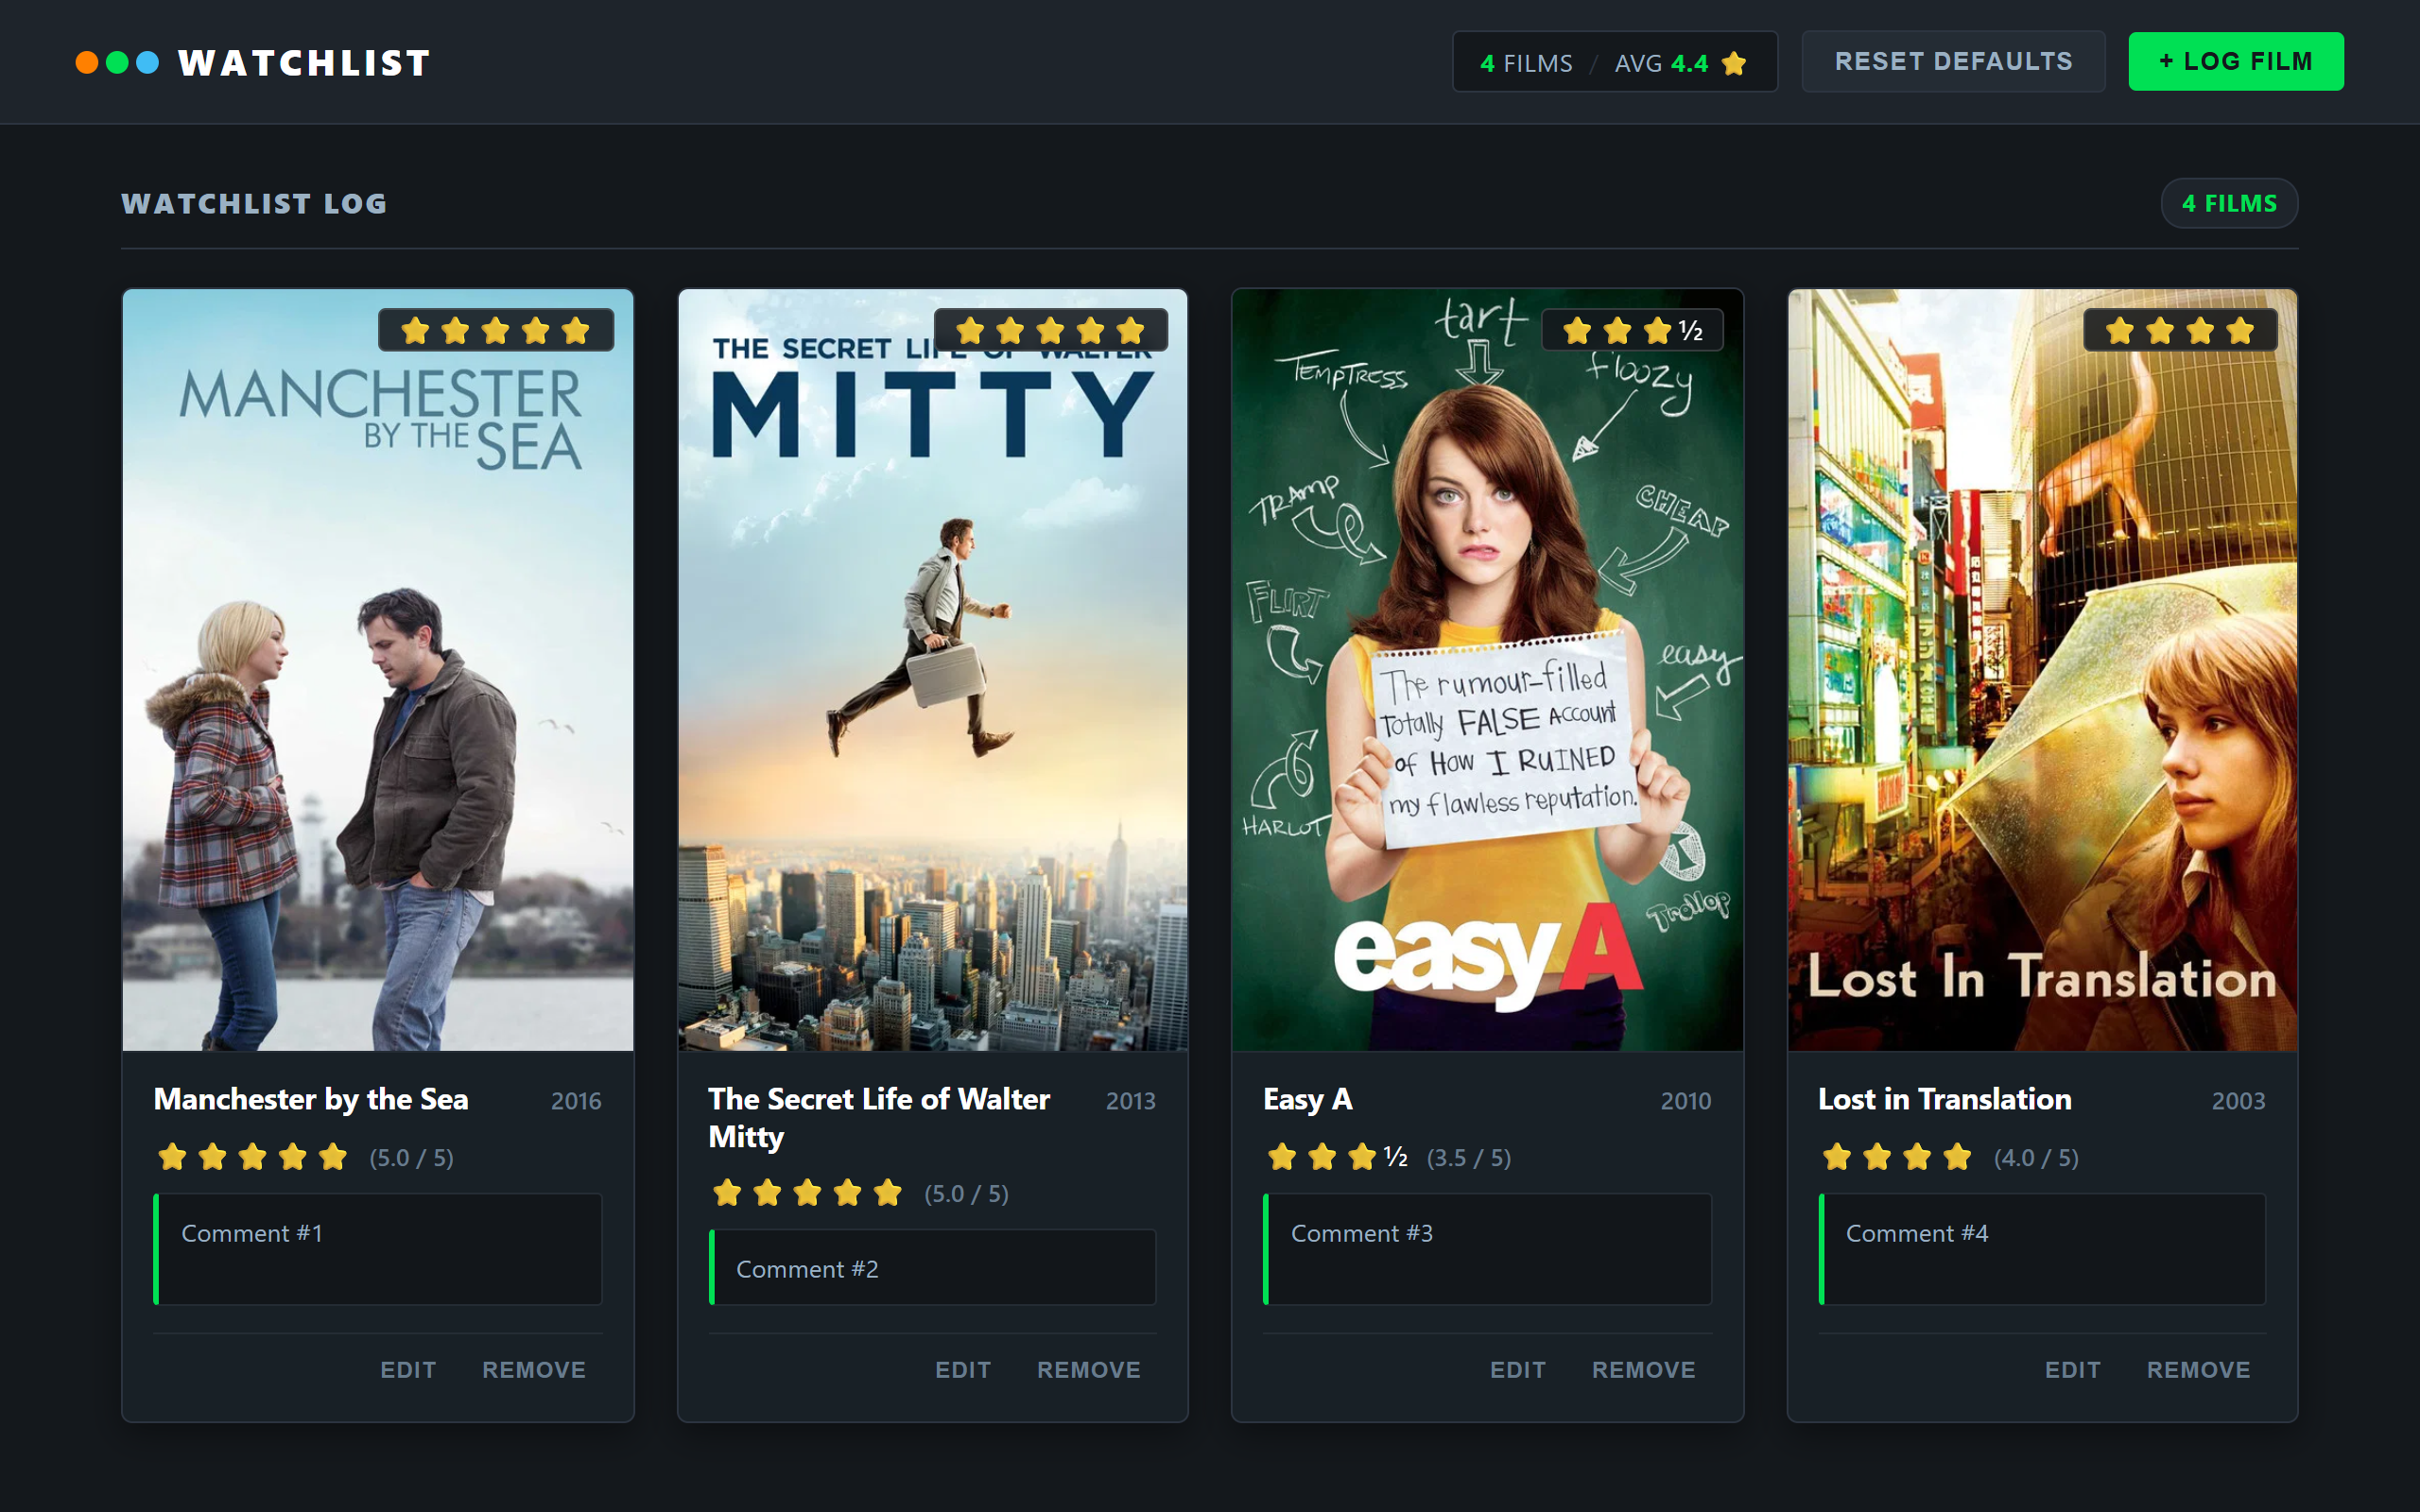
\includegraphics[width=0.96\textwidth,height=0.38\textheight,keepaspectratio]{screenshot1.png}
\end{figure}

\vspace{0.4cm}

\begin{figure}[H]
    \centering
    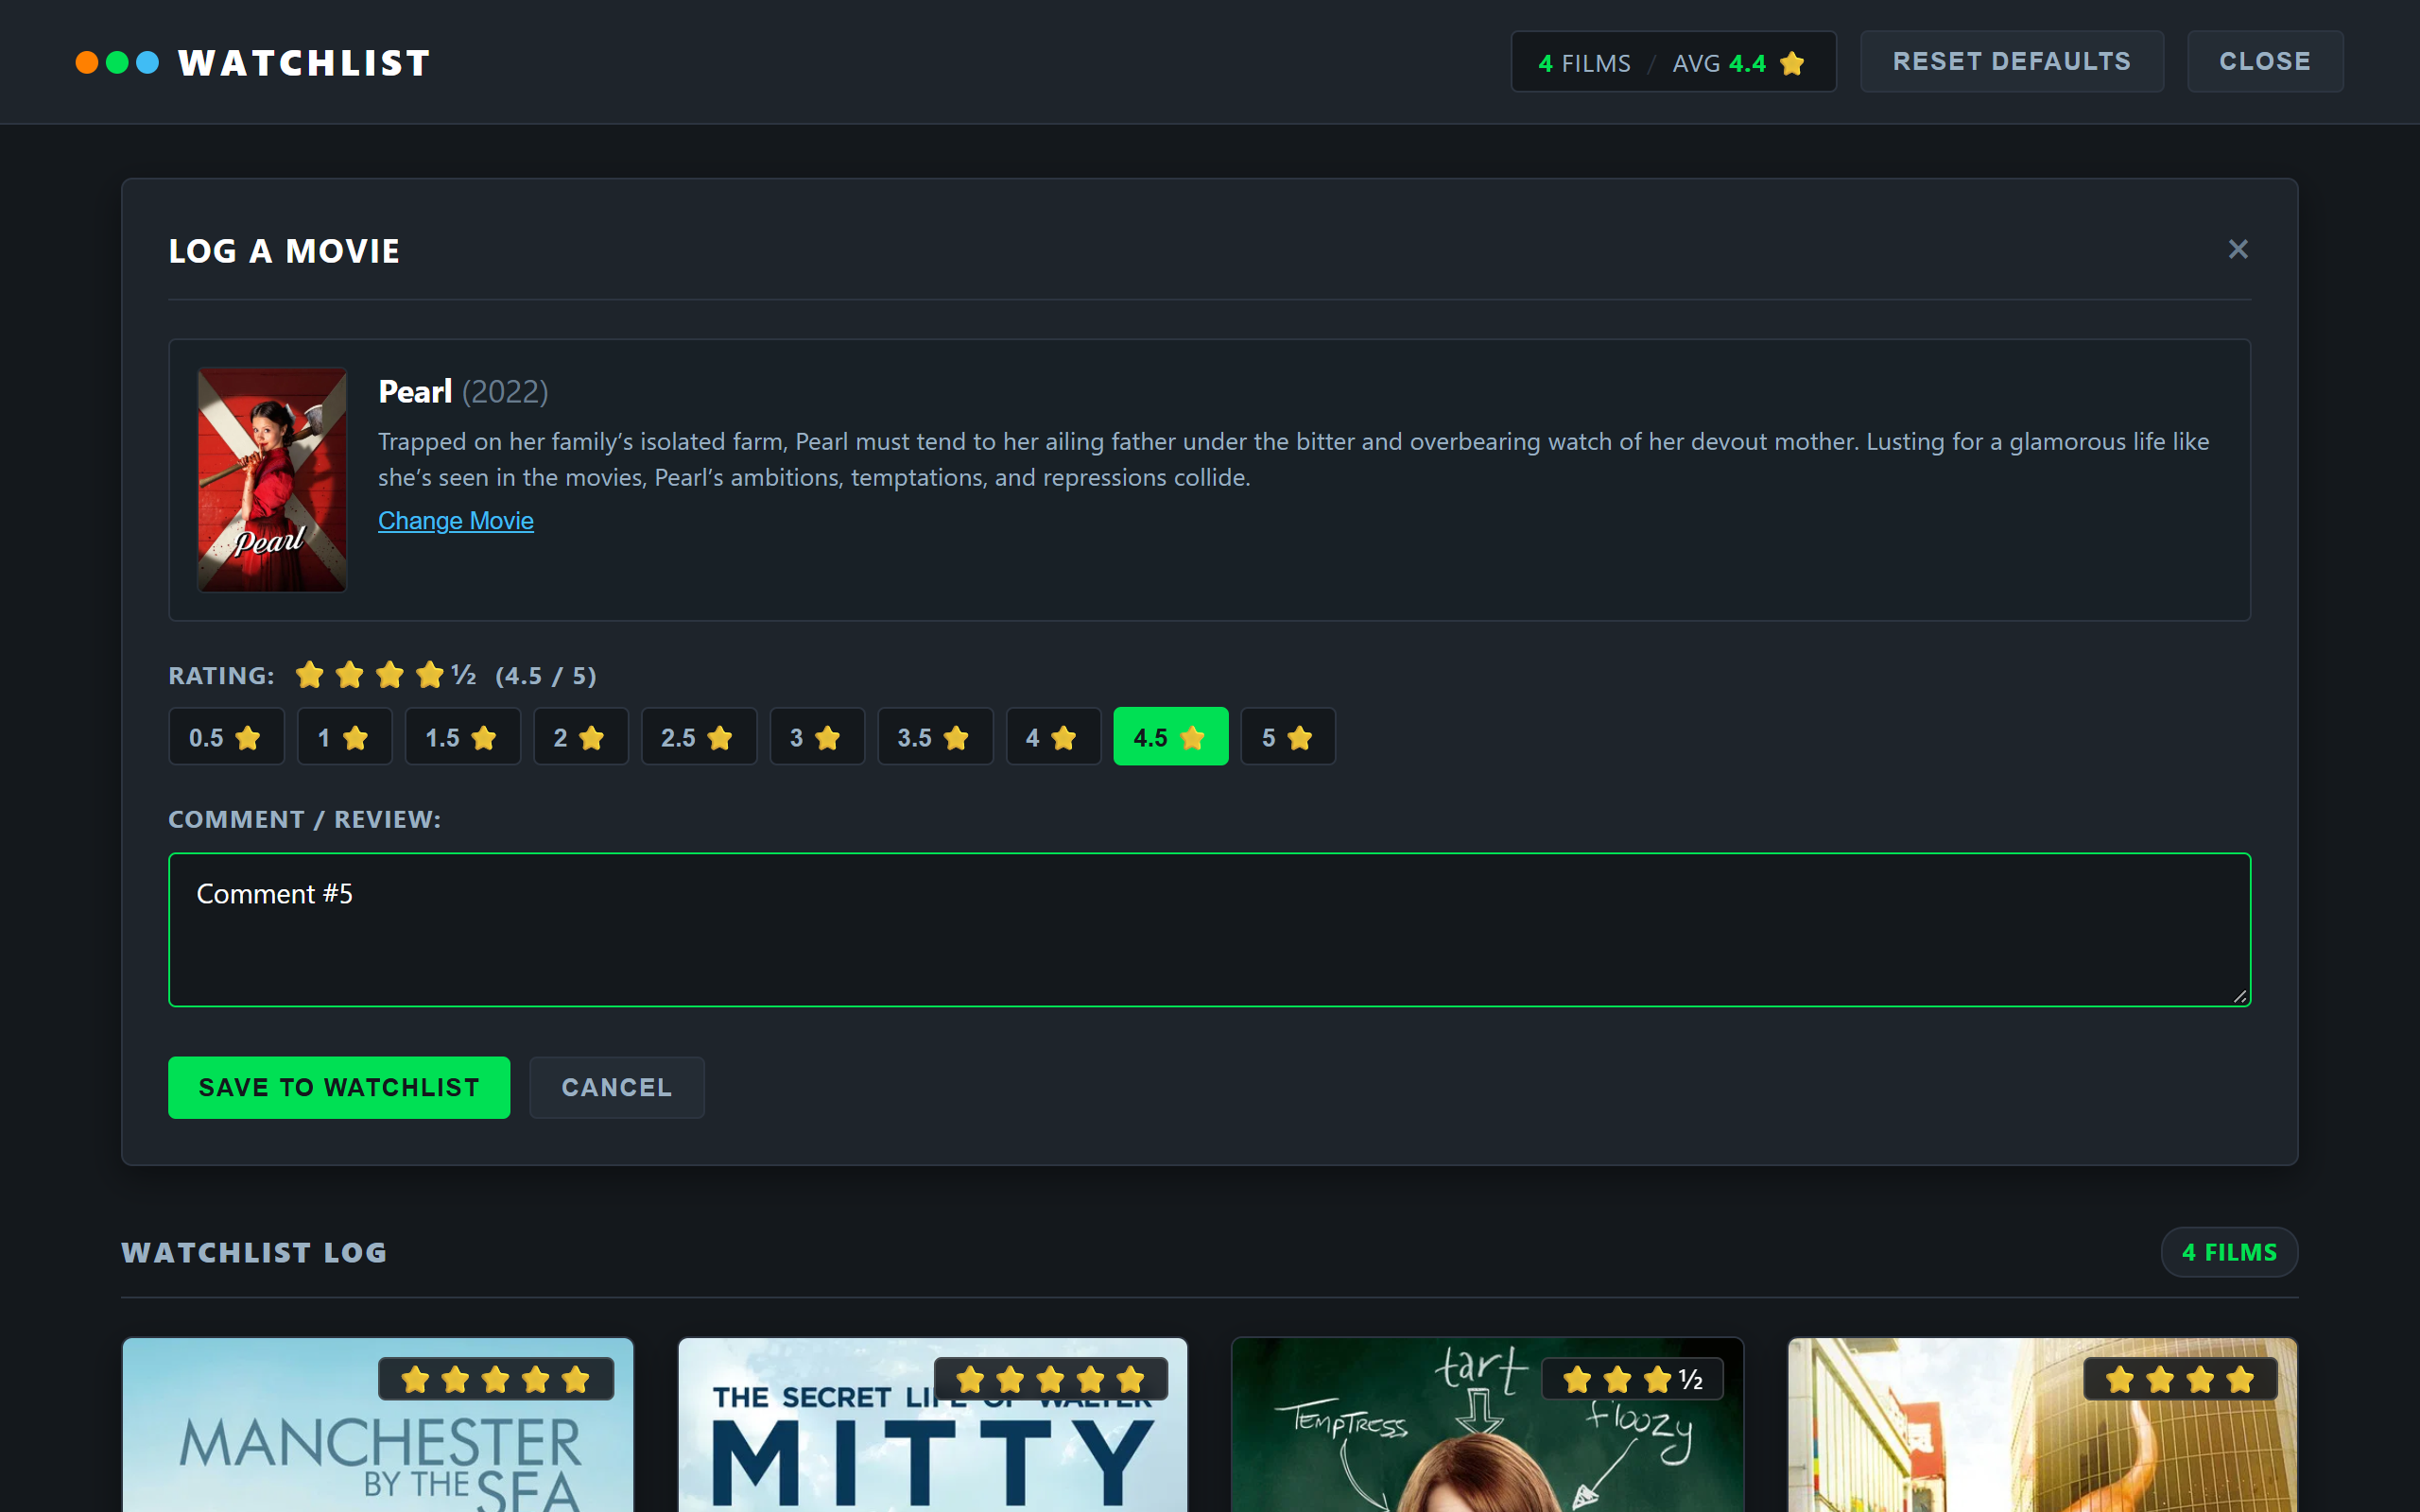
\includegraphics[width=0.96\textwidth,height=0.38\textheight,keepaspectratio]{screenshot2.png}
\end{figure}

% ---  Task Description  ---
\clearpage
\section*{Task Description}

\begin{itemize}
    \item The application uses a TMDB API key to fetch films and posters.
    \item The TMDB API key is kept safe in \texttt{.env}.
    \item The UI was inspired by Letterboxd.
\end{itemize}

\vspace{1cm}

\section*{Repository}
\noindent \url{https://github.com/Auipp/Web-Dev-Labs-Repo}

\vspace{1cm}

\section*{References}
\begin{enumerate}
    \item \url{https://stylr.dev/styles/letterboxd}
    \item \url{https://codepen.io/cycosta/pen/Pogepzw}
    \item \url{https://www.themoviedb.org/}
\end{enumerate}

\end{document}
